% Author: Till Tantau
% Source: The PGF/TikZ manual

\documentclass[landscape]{article}

\usepackage{pgf}
\usepackage{tikz}
\usetikzlibrary{arrows,automata}
\usepackage[latin1]{inputenc}
\usepackage{verbatim}
\usepackage{pdflscape}


\begin{document}

\hspace{-5cm}
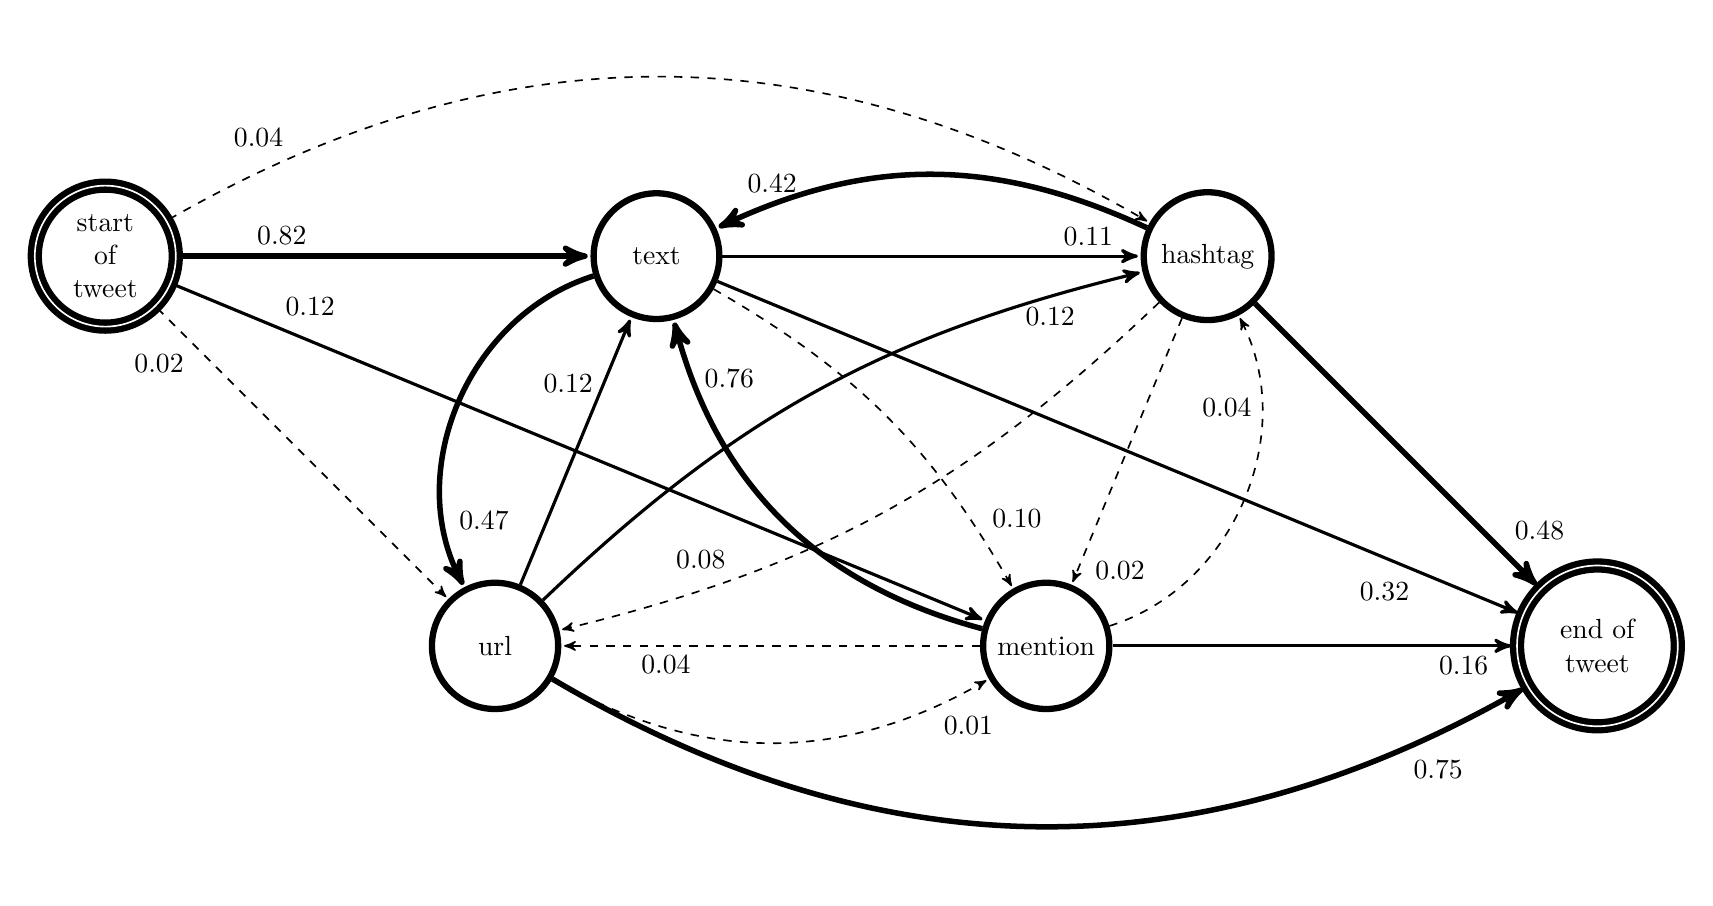
\begin{tikzpicture}[->,>=stealth',shorten >=1pt,auto,node distance=7cm,
                    semithick]
  \tikzstyle{every state}=[fill=white,draw=black,text=black,line width=.8mm, align=center]

  \node[state] (A) [text width=1cm,double]  {start of tweet};
  \node[state]         (B) [right of=A,text width=1.30cm] 	 {text};
  \node[state]         (C) [right of=B,text width=1.30cm] {hashtag};
  \node[state]         (E) [below right of=A,text width=1.30cm]       {url};
  \node[state]         (D) [right of=E,text width=1.30cm] {mention};
  \node[state]         (F) [right of=D,text width=1.60cm,double]       {end of tweet};
  
  \path   (C)	 	edge [ very near end,dashed]   									node {0.02}	 (D)
		  			edge [bend left=15,  near end,above left,dashed]  				node {0.08}	 (E)
		  	 		edge [bend right=25, very near end,above,line width=0.7mm]   	node {0.42}	 (B)
		  	 		edge [near start, very near end,line width=0.7mm]   			node {0.48}	 (F)
		  (D)	 	edge [bend right=50, near end, left,dashed]      				node {0.04}	 (C)
		  	 		edge [near start, near end,dashed]    							node {0.04}	 (E)
		  	 		edge [near start, very near end,below,line width=0.40mm]    	node {0.16}	 (F)
		  	 		edge [bend left, very near end,right,line width=0.7mm]    		node {0.76}	 (B)
		  (A)	 	edge [very near start, below left,dashed]   					node {0.02}	 (E)
		  	 		edge [bend left,very near start,dashed]  						node {0.04}	 (C)
		  	 		edge [very near start,line width=0.40mm]  						node {0.12}	 (D)
		  	 		edge [near start,line width=0.7mm]   							node {0.82}	 (B)
		  (B)	 	edge [bend left=15, very near end,dashed]  						node {0.10}	 (D)
		  	 		edge [very near end,line width=0.40mm]   						node {0.11}	 (C)
		  	 		edge [near start, very near end,below left,line width=0.40mm] 	node {0.32}	 (F)
		  	 		edge [bend right=50, very near end,line width=0.7mm]   			node {0.47}	 (E)
		  (E)	 	edge [bend right, very near end,dashed,below right]   			node {0.01}	 (D)
		  	 		edge [bend left=15, very near end,below,line width=0.40mm]  	node {0.12}	 (C)
		  	 		edge [near end,line width=0.40mm,left]  						node {0.12}	 (B)
		  	 		edge [bend right, very near end,below right,line width=0.7mm]  	node {0.75}	 (F);
  ;
\end{tikzpicture}
\end{document}

